\begin{frame}{Circuito ativo e configurações estudadas}
  \begin{columns}[c,onlytextwidth]
    \begin{column}{0.54\textwidth}
      \centering
      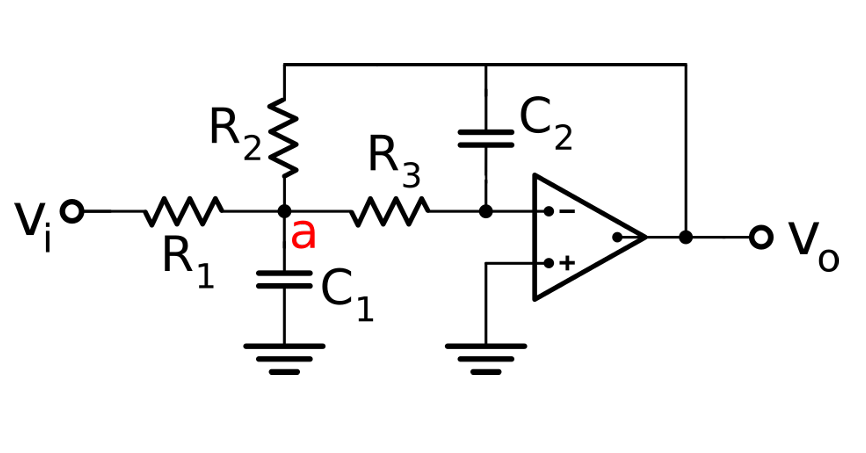
\includegraphics[width=\linewidth]{slides/img/circuito_passabaixa.png}

      \vspace{0.14cm}
      \scriptsize Topologia passa-baixa de realimentação múltipla.
    \end{column}
    \begin{column}{0.43\textwidth}
      \small
      \begin{block}{Componentes comuns}
        $C_1=100\,\mathrm{nF}$, $C_2=10\,\mathrm{nF}$\\
        $R_2=470\,\mathrm{k}\Omega$; alimentação: $\pm10\,\mathrm{V}$.
      \end{block}

      \begin{tabular}{lcc}
        \toprule
        & Circuito 1 & Circuito 2 \\
        \midrule
        $R_1$ & $47\,\mathrm{k}\Omega$ & $470\,\mathrm{k}\Omega$ \\
        $R_3$ & $470\,\mathrm{k}\Omega$ & $47\,\mathrm{k}\Omega$ \\
        \bottomrule
      \end{tabular}

      \begin{alertblock}{Alteração investigada}
        A troca entre $R_1$ e $R_3$ modifica o ganho e a posição dos polos,
        preservando a topologia.
      \end{alertblock}
    \end{column}
  \end{columns}
\end{frame}
